% !TeX TS-program = xelatex
% !BIB TS-program = bibtex

% Full instructions available at:
% https://github.com/pcafrica/focus-beamertheme

\documentclass{beamer}
% \usetheme{focus}
\usetheme[numbering=minimal]{focus}
% \usetheme[numbering=minimal, totalframenumbering=no]{focus}
% \usetheme[numbering=fullbar]{focus}
\definecolor{main}{RGB}{45, 45, 45}
% \definecolor{main}{HTML}{1A1A1A}
\definecolor{background}{RGB}{242, 241, 239}
% \definecolor{background}{HTML}{F5F5F5}

\usepackage{geometry}
\geometry{paperwidth=16cm, paperheight=9cm}
\usepackage{tikz}
\usepackage{amsthm,amsmath,bbm,amsfonts,amssymb, mathrsfs}
\usepackage{mathtools}

% math expressions
\def \bc {\textbf{c}}
\def \bz {\textbf{z}}
\def \bZ {\textbf{Z}}
\def \bA {\textbf{A}}
\def \ba {\textbf{a}}
\def \bX {\textbf{X}}
\def \bY {\textbf{Y}}
\def \wY {\widetilde{Y}}
\def \bI {\textbf{I}}
\def \bS {\textbf{S}}
\def \bR {\textbf{R}}
\def \bU {\textbf{U}}
\def \bO {\textbf{O}}
\def \bx {\textbf{x}}
\def \bw {\textbf{w}}
\def \beps {\boldsymbol{\varepsilon}}
\def \balpha {\boldsymbol{\alpha}}
\def \bphi {\boldsymbol{\phi}}
\def \boeta {\boldsymbol{\eta}}
\def \bgamma {\boldsymbol{\gamma}}
\def \btheta {\boldsymbol{\theta}}
\def \bQ {\textbf{Q}}
\def \bD {\textbf{D}}
\def \bpsi {\textbf{\psi}}
\def \bbE {\mathbb{E}}

% tikz stuff
\usetikzlibrary{positioning, calc, shapes.geometric, shapes.multipart, shapes, arrows.meta, arrows, 	decorations.markings, external, trees}

\tikzstyle{Arrow} = [
thick,
decoration={
	markings,
	mark=at position 0.99 with {  % fix bug with tikz arrow head interference with decoration
		\arrow[thick]{latex}
	}
},
shorten >= 3pt, preaction = {decorate}
]
\tikzstyle{BiArrow} = [
thick,
decoration={
	markings,
	mark=at position 0.99 with {  % fix bug with tikz arrow head interference with decoration
		\arrow[thick]{latex}
	}
},
shorten >= 3pt, preaction = {decorate}
]
\tikzstyle{RedArrow} = [
red, 
line width = 0.5mm,
decoration={
	markings,
	mark=at position 0.99 with {
		\arrow[line width = 0.5mm,red]{latex}
	}
},
shorten >= 3pt, preaction = {decorate}
]

\tikzstyle{BlueArrow} = [
blue, 
line width = 0.5mm,
decoration={
	markings,
	mark=at position 0.99 with {
		\arrow[line width = 0.5mm,blue]{latex}
	}
},
shorten >= 3pt, preaction = {decorate}
]

\tikzstyle{Dashed} = [
thick,dashed,
decoration={
	markings,
	mark=at position 0.99 with {  % fix bug with tikz arrow head interference with decoration
		\arrow[thick]{latex}
	}
},
shorten >= 3pt, preaction = {decorate}
]

\tikzset{
    BiArrow/.style={
        thick,
        decoration={
            markings,
            mark=at position 0.99 with {
                \arrow[thick]{latex}
            },
            mark=at position 0 with {
                \arrow[thick]{latex}
            }
        },
        shorten >= 3pt,
        preaction = {decorate}
    }
}


\title{Estimating Causal Effects Using \texorpdfstring{\\}{,} Proxy Interference Networks}
% \subtitle{Subtitle}
\author{Bar Weinstein \texorpdfstring{\\}{,} Daniel Nevo}
\titlegraphic{\includegraphics[scale=0.22]{figs/noisy_networks.png}}
\institute{Statistics \& OR \\ Tel Aviv University}
\date{IDSAI 2025}

% Footline info is printed only if [numbering=fullbar].
%\footlineinfo{Custom footline text}



\begin{document}
    \begin{frame}
        \maketitle
    \end{frame}
    
    % Use starred version (e.g. \section*{Section name})
    % to disable (sub)section page.
    \begin{frame}{Background}
        \large
        \begin{itemize}
            \item<1-> \textbf{Causal Inference}. Estimate the effect of treatment on an outcome. 
            \vspace{0.2cm}
            \item<1-> \textbf{Interference}. Treatment of one unit affect the outcomes of others.
            \vspace{0.2cm}
            \item<1->  Treatments spreads through a network.
            \begin{itemize}
                \item Nodes: units; Edges: magntiude of pairwise interfernce.
            \vspace{0.2cm}
            \end{itemize}
            \item<2-> Examples:
                \begin{itemize}
                    \item \emph{Social networks.} Transmission of information, behavior, encouragements, etc.
                    \vspace{0.05cm}
                    \item \emph{Epidemiology.} Mitigating spread of infectious diseases or addictive drugs.
                    \vspace{0.05cm}
                    \item A/B testing in marketplaces.
                \end{itemize} 
        \end{itemize}
    \end{frame}

    \begin{frame}[t]
        \begin{figure}[t]
            \centering
            \includegraphics[width=0.65\textwidth]{figs/connected_net.png}
            % \caption{Plain frame with a figure.}
        \end{figure}
    \end{frame}

    \begin{frame}{The Challenge}
        \large
        \begin{itemize}
            \item<1-> Accurately measuring social networks is challenging.
            \vspace{0.2cm}
            \item<1-> We observe only proxy measurements of the true network.
            \begin{itemize}
                \item Measurements error.
                \item Multiple sources of data.
                \item Multilayer networks.
            \end{itemize}
            \vspace{0.2cm}
            \item<1-> True network remains latent.
        \end{itemize}
        \vspace{.5cm}
        \pause
        \begin{center}
            \Large
            \textbf{How can we estimate causal effects using proxy networks?}
        \end{center}
    \end{frame}

    \begin{frame}[t]
        \begin{figure}[t]
            \centering
            \includegraphics[width=0.8\textwidth]{figs/noisy_networks.png}
            % \caption{Plain frame with a figure.}
        \end{figure}
    \end{frame}
    
    \begin{frame}{Illustrative Example -- Paluck et al. (2016)}
        \large
        \begin{itemize}
            \item<1-> Field experiement in 56 middle-schools.
            \vspace{0.2cm}
            \item<1-> Study how anti-conflict education spread through social networks.
            \vspace{0.2cm}
            \item<1-> Measured social networks using self-reported friendships.
            \begin{itemize}
                \item Bi-layer networks: frequently interacted and best friends.
                \vspace{0.05cm}
                \item Measured at pre- and post-intervention period.
            \end{itemize} 
            \vspace{0.2cm}
            \item<2-> Which of the networks, if any, is the true network?
            \vspace{0.2cm}
            \item<2-> \textbf{Objective:} Estimate the intervention effects using the proxy networks.
        \end{itemize}
    \end{frame}
    
    \begin{frame}{Formal Setup}
        \large 
        \begin{itemize}
            \item Finite population $i \in \{1,\ldots, N\}$.
            \vspace{0.2cm}
            \item Treatments: $\bZ \in \{0,1\}^N$.
            \vspace{0.2cm}
            \item Outcomes: $\bY \in \mathbb{R}^N$.
            \vspace{0.2cm}
            \item Covariates/features: $\bX$.
            \vspace{0.2cm}
            \item True interference network: $\bA^\ast \in \{0,1\}^{N \times N}$.
            \vspace{0.2cm}
            \item Proxy networks: $\bA=\big(\bA^1,\ldots,\bA^B\big)$.
        \end{itemize}
    \end{frame}

    \begin{frame}{Structural Causal Model}
        \large
        \begin{itemize}
            \item<1-> Population-level directed acyclic graph (DAG):
            \begin{figure}[hbtp]
                \centering
                  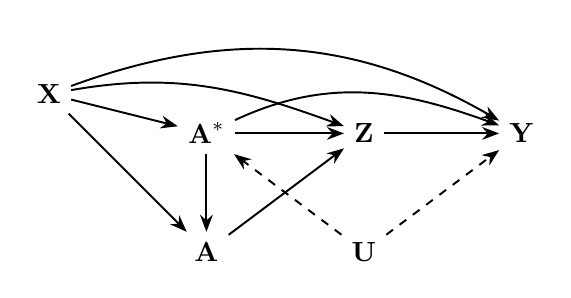
\begin{tikzpicture}[>=Stealth,line width=.7pt]
                    \node (X) at (0, 2.5) {$\bX$};
                    \node (A*) at (2, 2) {$\bA^\ast$};
                    \node (A) at (2, .5) {$\bA$};
                    \node (Z) at (4, 2) {$\bZ$};
                    \node (Y) at (6, 2) {$\bY$};
                    \node (U) at (4, .5) {$\bU$};
                    \draw[->] (X) -- (A*);
                    \draw[->] (X) -- (A);
                    \draw[->] (X) to [out=10,in=160] (Z);
                    \draw[->] (X) to [out=20,in=150] (Y);
                    \draw[->] (A*) -- (Z);
                    \draw[->] (A*) -- (A);
                    \draw[->] (Z) -- (Y);
                    \draw[->] (A*) to [out=25,in=160] (Y);
                    \draw[->] (A) -- (Z);
                    \draw[->, dashed] (U) to (A*);
                    \draw[->, dashed] (U) to (Y);
                  \end{tikzpicture}
              \end{figure}
            \item<2-> Requires probabilistic models:
            \begin{enumerate}
                \normalsize
                \item \emph{True network.} $p\big(\bA^\ast \vert \bX, \btheta \big)$.
                \vspace{0.1cm}
                \item \emph{Proxy networks.} $p\big(\bA \vert \bA^\ast, \bX, \bgamma \big)$.
                \vspace{0.1cm}
                \item \emph{Outcomes.} $p\big(\bY \vert \bZ, \bA^\ast, \bX, \boeta \big)$.
            \end{enumerate} 
            % \vspace{0.2cm}
            % \item<3-> Outcome often simplified to
            % \normalsize $p\big(Y_i \vert Z_i,\bX_i, \phi_1(\bZ_{-i},\bA^\ast), \phi_2(\bX_{-i},\bA^\ast),\phi_{3,i}(\bA^\ast)\big)$.
        \end{itemize}
    \end{frame}

    \begin{frame}{Causal Estimands}
        \large
        Causal effects are the impact of hypothetical interventions on $\bZ$. \\
        \vspace{0.1cm}
        Can be viewed as population-level treatment assignment policies.
        \vspace{0.3cm}
        \pause
        \begin{enumerate}
            \item \textbf{Static.} $\bbE\big[Y_i \vert do(\bZ=\bz),\bX,\bA^\ast\big]$.
            \begin{itemize}
                \item Treating all ($\bz=\boldsymbol{1}$) versus none ($\bz = \boldsymbol{0}$).
            \end{itemize}
            \vspace{0.2cm}
            \item \textbf{Dynamic.} $\bbE\big[Y_i \vert do(\bZ=h(\bX,\bA^\ast)),\bX,\bA^\ast\big]$.
            \begin{itemize}
                \item Treating units with specific features, e.g., above certain age. 
            \end{itemize}
            \vspace{0.2cm}
            \item \textbf{Stochastic.} $\bbE_{\pi_\alpha(\bZ)}\bbE\big[Y_i \vert do(\bZ),\bX,\bA^\ast\big]$.
            \begin{itemize}
                \item Expected impact of randomly treating $\alpha_1$ vs $\alpha_0$ percent of units.
            \end{itemize}
        \end{enumerate}
    \end{frame}

    \begin{frame}{Bayesian Inference}
        \large
        \begin{itemize}
            \item<1-> Observed data $\bO = (\bY,\bZ,\bX,\bA)$. Latent variables $(\bA^\ast, \eta,\gamma,\theta)$.
            \vspace{0.2cm}
            \item<2-> Posterior distribution:
            \begin{equation*}
                % \label{eq:observed.posterior}
                \begin{split}
                    p(\bA^\ast, \eta,\gamma,\theta \vert \bO) 
                        \propto
                    &\;
                    p(\bY \vert \bZ,\bA^\ast,\bX,\boeta) p(\boeta) 
                    \\ & \times
                    p(\bA \vert \bA^\ast, \bX,\bgamma) p(\bgamma)
                    \\ & \times 
                    p(\bA^\ast \vert \bX,\btheta) p(\btheta).
                \end{split}
            \end{equation*} 
            \item<3-> Mixed space of continuous $(\eta,\gamma,\theta)$ and discrete $\bA^\ast$. Discrete have $\mathcal{O}(N^2)$ terms!
            \item<4-> Propose two sampling schemes:
            \begin{enumerate}
                \item \emph{Modularization.} ``break" the posterior into smaller, more manageable parts.
                \vspace{0.1cm}
                \item \emph{Gibbs.} Iterate between continuous and discrete. Sample discrete with \emph{Local Informed Proposals}.
            \end{enumerate} 
        \end{itemize}
    \end{frame}

    \begin{frame}{Simulations}
        Two figures: MAPE of estimated treatment effects and MAE of exposure mapping.        
    \end{frame}

    \begin{frame}{Data Analysis}
        Results of Paluck et al. (2016) analysis.
    \end{frame}

    
\setbeamertemplate{caption}[numbered]
    \begin{frame}{Figures and Tables}
        \begin{columns}
            \column{0.4\textwidth}
                \begin{figure}
                    \centering
                    \includegraphics{focus-logo.pdf}
                    \caption{Figure caption.}
                    \label{fig:focuslogo}
                \end{figure}
                
            \column{0.6\textwidth}
                \begin{table}
                    \centering
                    \begin{tabular}{rcc}
                         & Heading 1 & Heading 2 \\\hline
                        Row 1 & \(v_{11}\) & \(v_{12}\) \\
                        Row 2 & \(v_{21}\) & \(v_{22}\) \\
                        Row 3 & \(v_{31}\) & \(v_{32}\) \\
                    \end{tabular}
                    \caption{Table caption.}
                    \label{tab:demo}
                \end{table}
        \end{columns}
    \end{frame}
    
    \begin{frame}[focus]
        Thanks for using \textbf{Focus}!
    \end{frame}
    
    \appendix
    \begin{frame}{References}
        \nocite{*}
        \bibliography{focus-demo_bibliography}
        \bibliographystyle{plain}
    \end{frame}
    
    \begin{frame}{Appendix}
        More math details.
    \end{frame}
\end{document}
